\subsection{Image Zonal Anatomy Segmentation and 3D Model Rendering}
Axial MR T2WI images were manually segmented using the smooth polygon tool in
ITK-SNAP~\cite{Yushkevich2006}, using unique labels for the PZ, CG and AFS. The
gland was segmented from base to apex.  The base was identified below the
bladder, and subsequent images were segmented until the last slice with visible
prostatic tissue was identified caudally. The CG and urethra, PZ and AFS were
segmented independently according to their well-established anatomical
characteristics on
T2WI.~\cite{Barentsz2012,Jung2012,Poon1985,Hricak2007,Bonekamp2011} The PZ was
identified by its homogenous high signal intensity on T2WI, which is usually
similar to that of the nearby periprostatic fat. The CG was visualized and
delineated based on its heterogeneous and lower signal intensity as well as its
location (Figure~\ref{fig:mr_anatomy}). The urethra was included in the CG
segmentation. Although not readily visible on every case, the AFS was
identified by its low T2 signal intensity and its location anterior to the
central gland. 

Figure~\ref{fig:mr_anatomy} shows the anatomic zones and some anatomic
orientation labels in the prostate of a representative study subject MR T2WI.  The
zonal anatomy of the prostate was manually segmented
(Figure~\ref{fig:mr_segs_vol}, bottom left) across the image stack, and 3D
models of the zonal anatomy volumes were rendered
(Figure~\ref{fig:mr_segs_vol}, top).

\begin{figure}
\centering
\begin{tabular}{ccc}
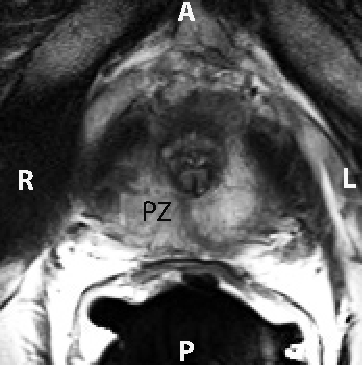
\includegraphics[width=0.29\linewidth]{figs/mr_anatomy/T2_apex} &
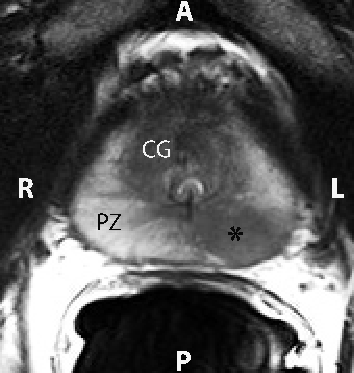
\includegraphics[width=0.275\linewidth]{figs/mr_anatomy/T2_midgland} &
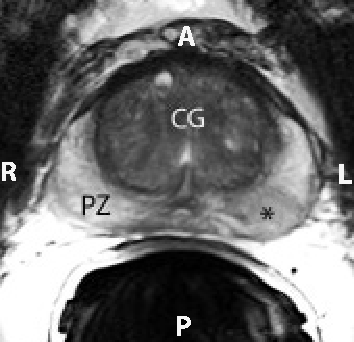
\includegraphics[width=0.3\linewidth]{figs/mr_anatomy/T2_base} \\
(a) MR T2WI Apex & (b) MR T2WI Mid-gland & (c) MR T2WI Base \\
\end{tabular}
\caption{Axial T2-weighted MR images of the prostate show the apex (a),
    mid-gland (b), and base (c).  The peripheral zone (PZ) is of higher signal
    intensity than the central gland (CG), the latter which is composed of the
    central zone and the transitional zone. The apex (a) is composed mostly of
    PZ glandular tissue and the urethra is seen at the level of the mid-gland as
    an inverted ``U'' (b). Note the area of hypointense signal in the
    peripheral zone at the mid-gland and base (asterisk, b and c), which
    represents a prostatic tumor.  The posterior (P) aspect of the prostate is
    adjacent to the endorectal coil, and the right (R)-to-left (L) extent of
    the prostate is referred to as the lateral-to-lateral axis in the subsequent
    analysis.}
\label{fig:mr_anatomy} 
\end{figure}


\begin{figure}[htb!]
\centering
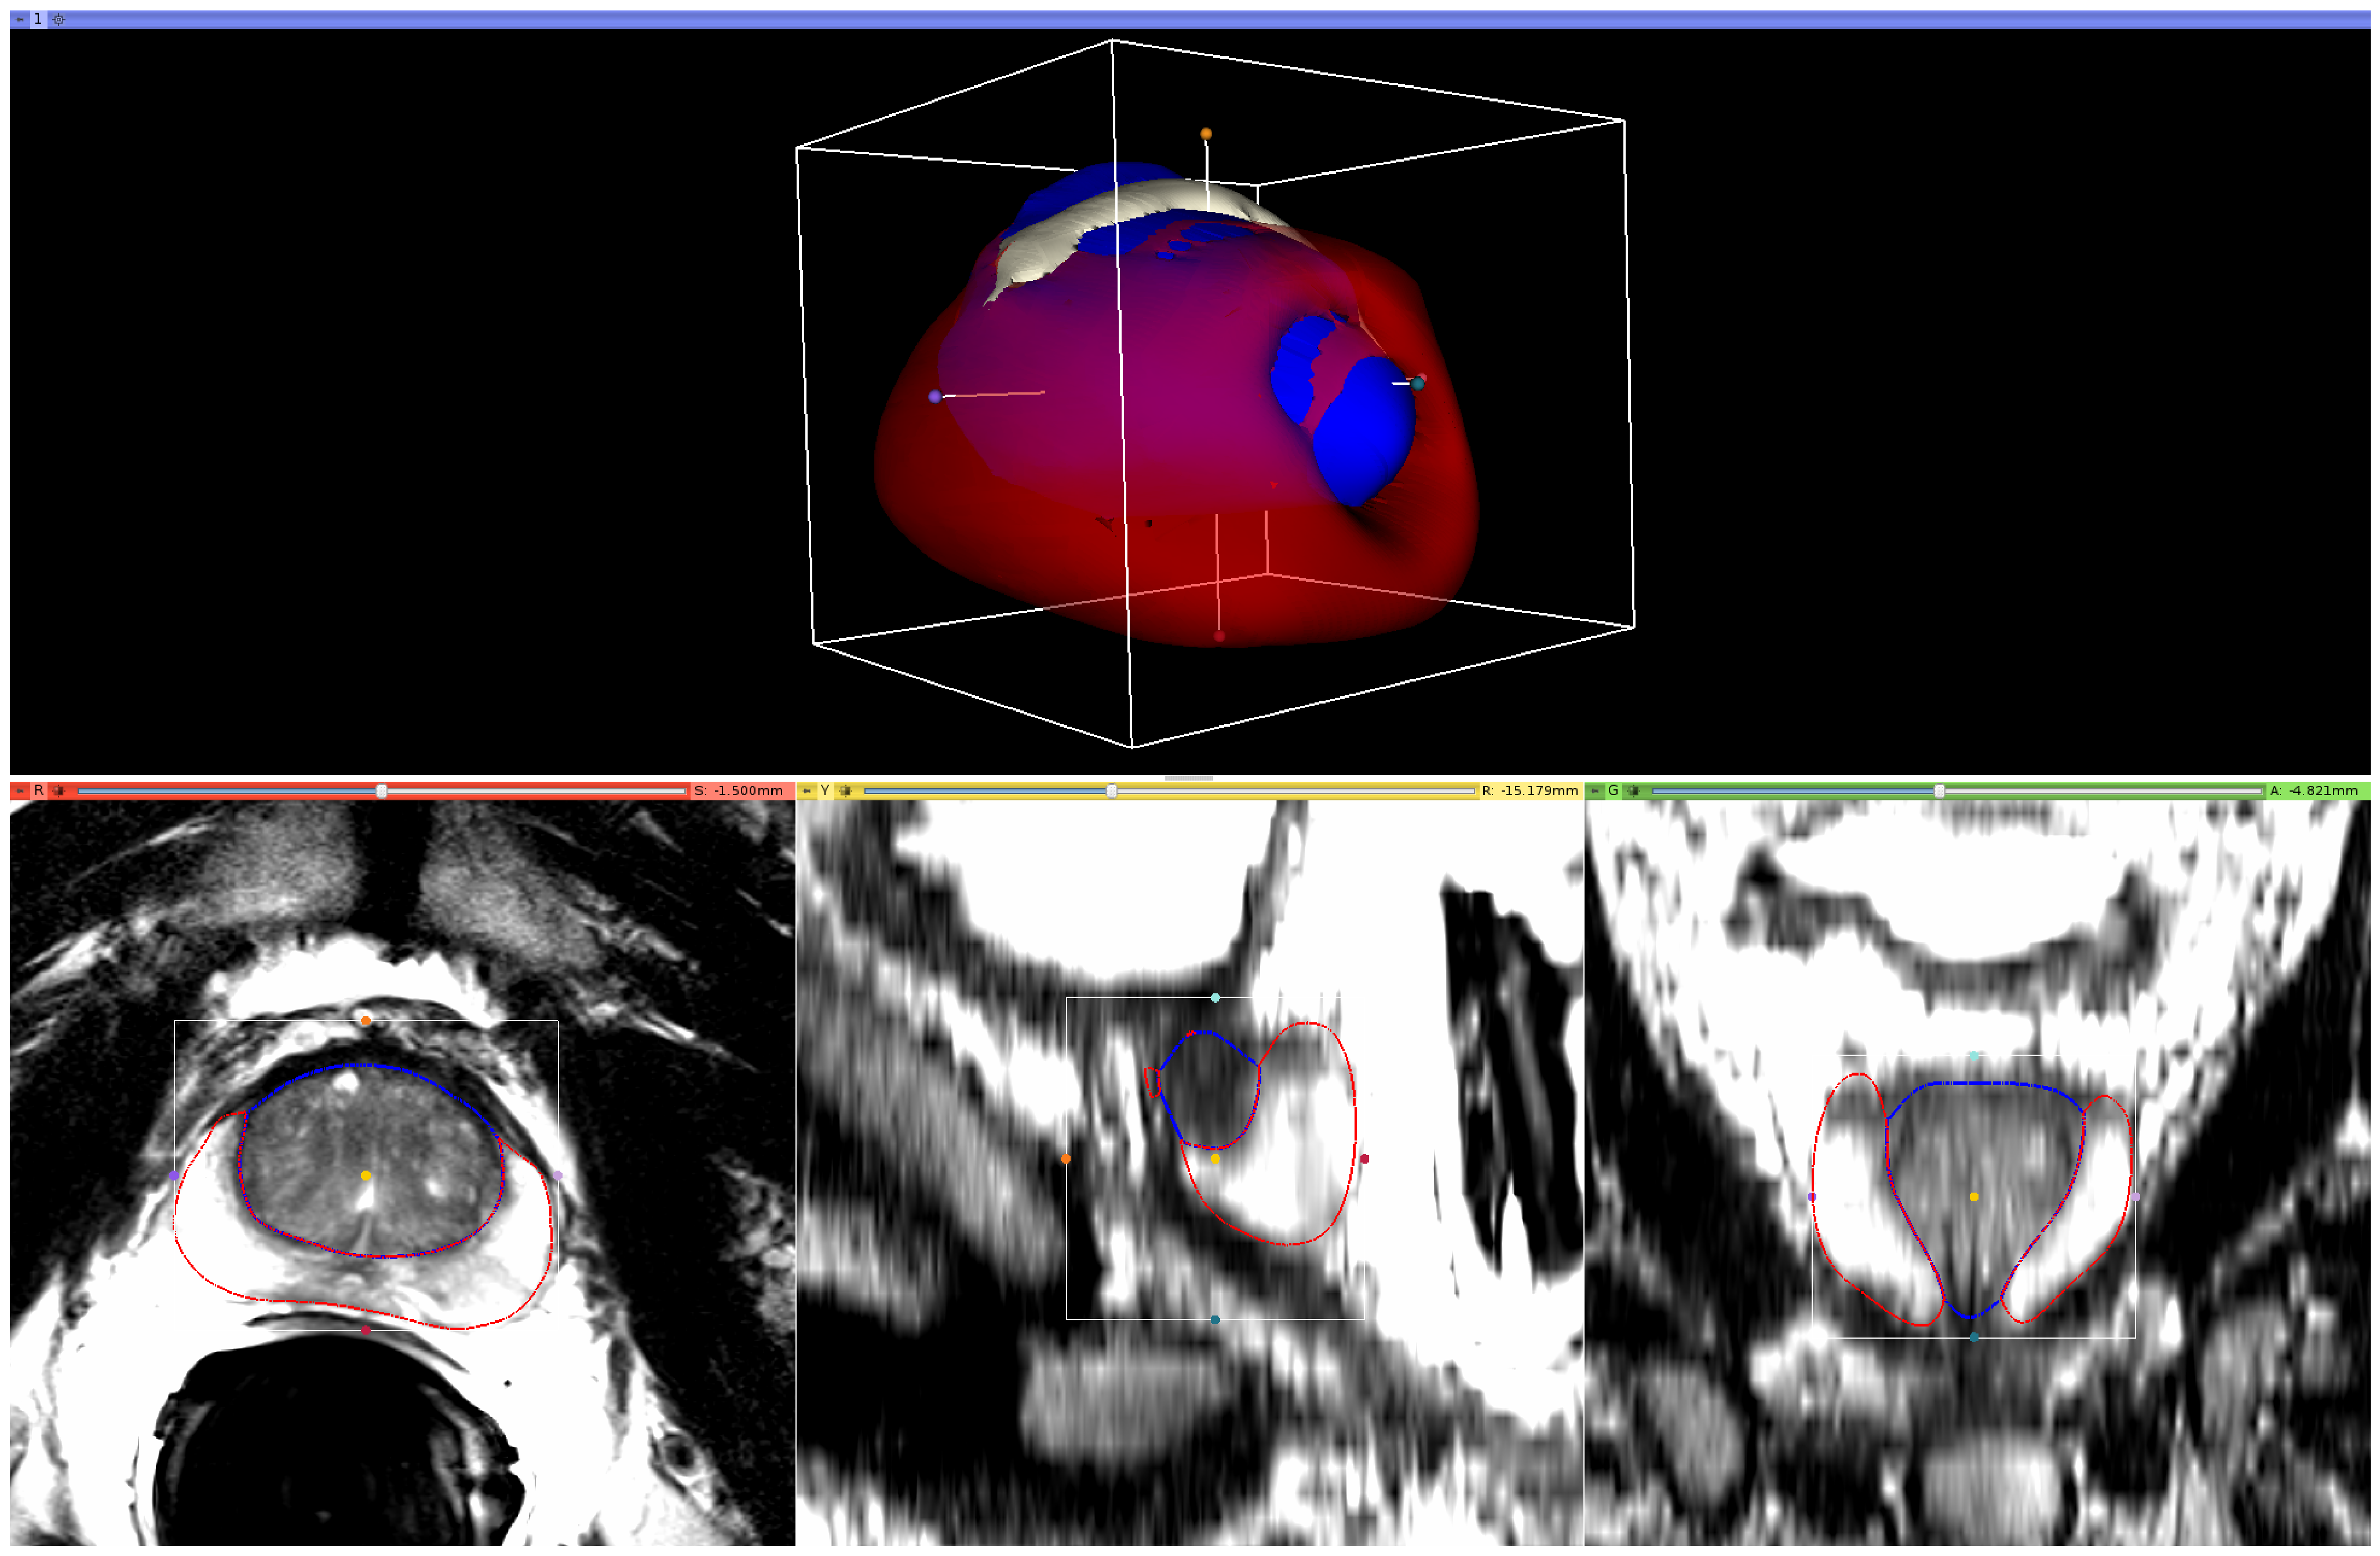
\includegraphics[width=1.0\textwidth]{figs/MR_P79_SegsVol.eps}
\caption{Representative MR T2WI segmentations and rendered volume performed in
    3D Slicer, with the peripheral zone (PZ) being delineated in red, the
    central gland (CG) being delineated in blue, and the anterior fibromuscular
    stroma (AFS) being shown in gray.  The AFS was combined with the PZ for
    quantitative analyses shown herein.  The native imaging plane for
    segmentation is the axial view, shown in the bottom left image.  The bottom
    middle and right images show the projections of the rendered model segment
    outlines in the sagital and coronal views, respectively.}
\label{fig:mr_segs_vol} 
\end{figure}


ARFI images were segmented using a similar procedure to the MR images.  B-mode
images were used to segment the prostate capsules since contrast between the
peripheral zone and the periprostatic fat can be low, and poor displacement SNR
can be present along the anterior aspect of the prostate in ARFI images, making
it difficult to delineate that boundary.  The central gland was segmented as a
stiffer region, relative to the peripheral zone, in the center of the prostate.

\begin{figure}[htb!]
\centering
\begin{tabular}{c}
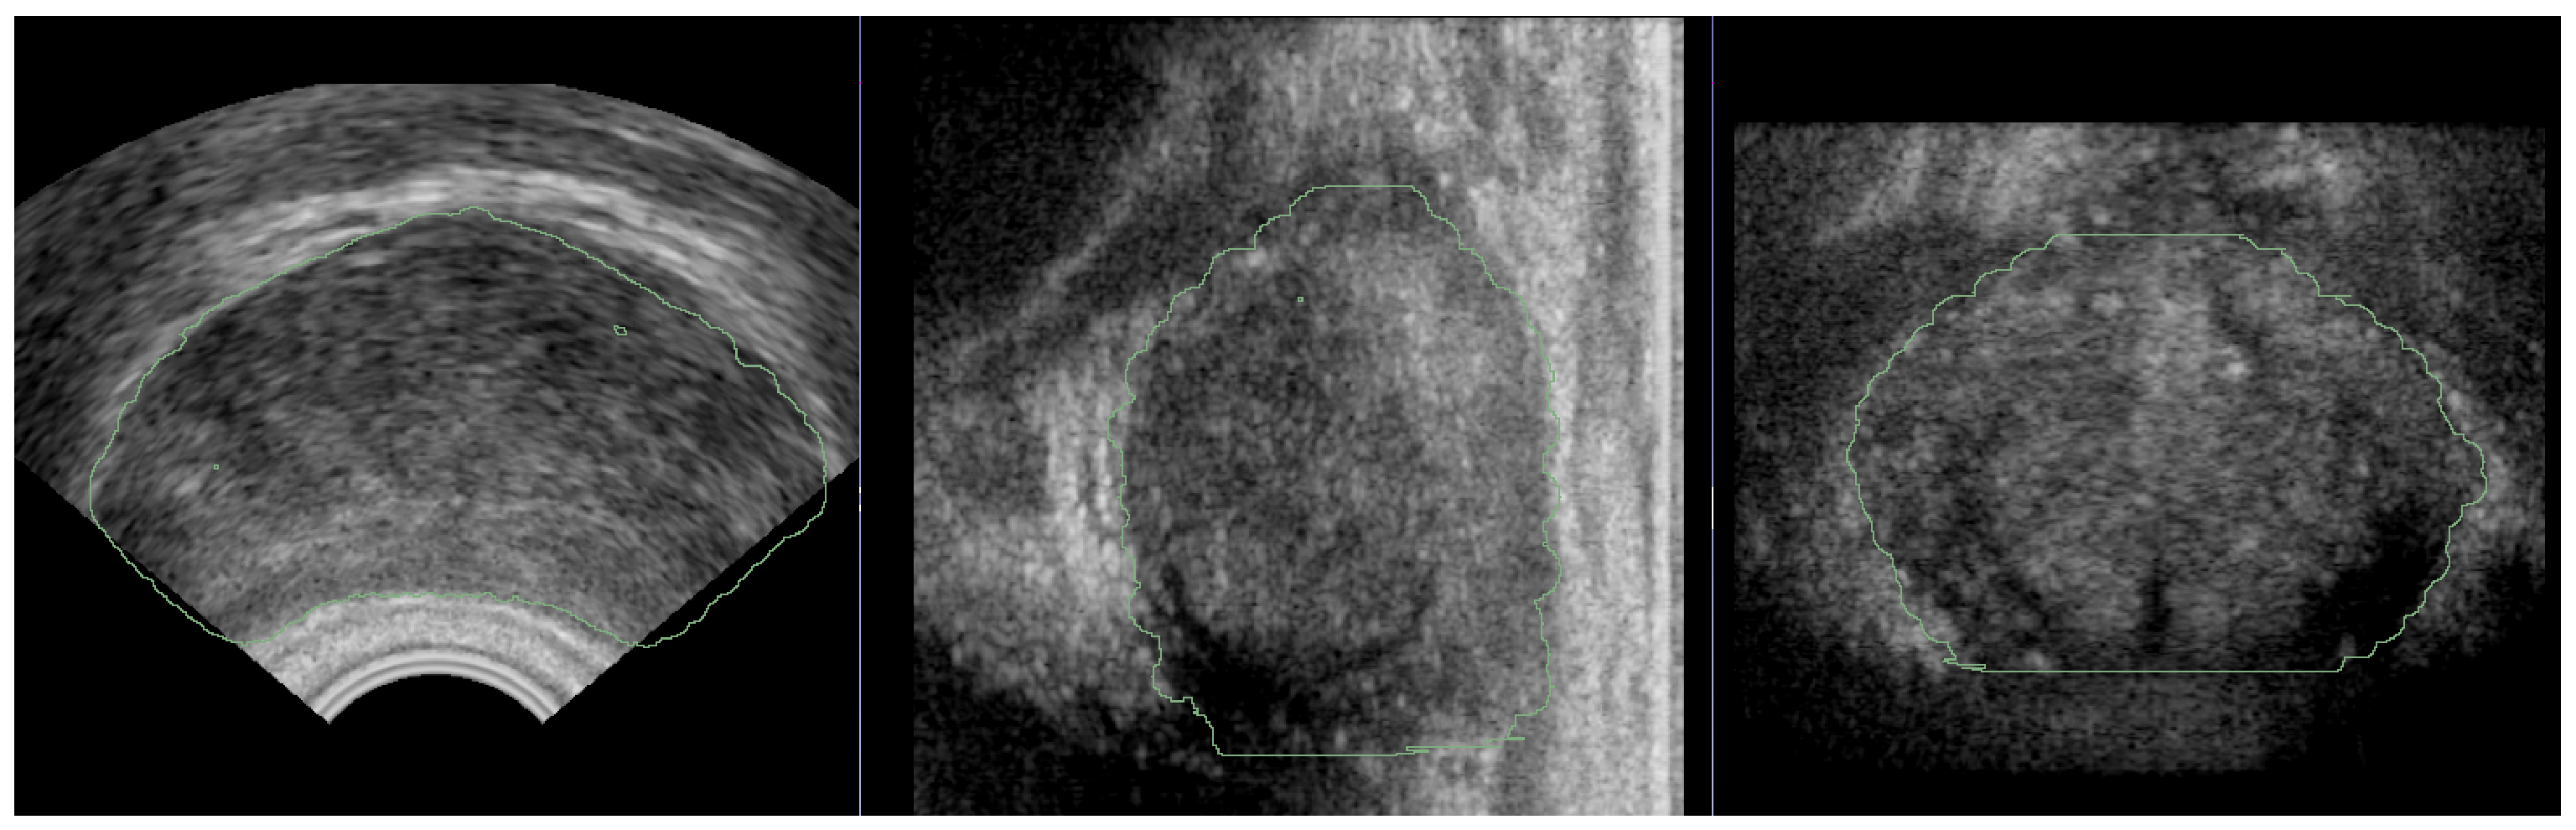
\includegraphics[width=1.0\textwidth]{figs/Bmode_CapsuleSegs.eps} \\
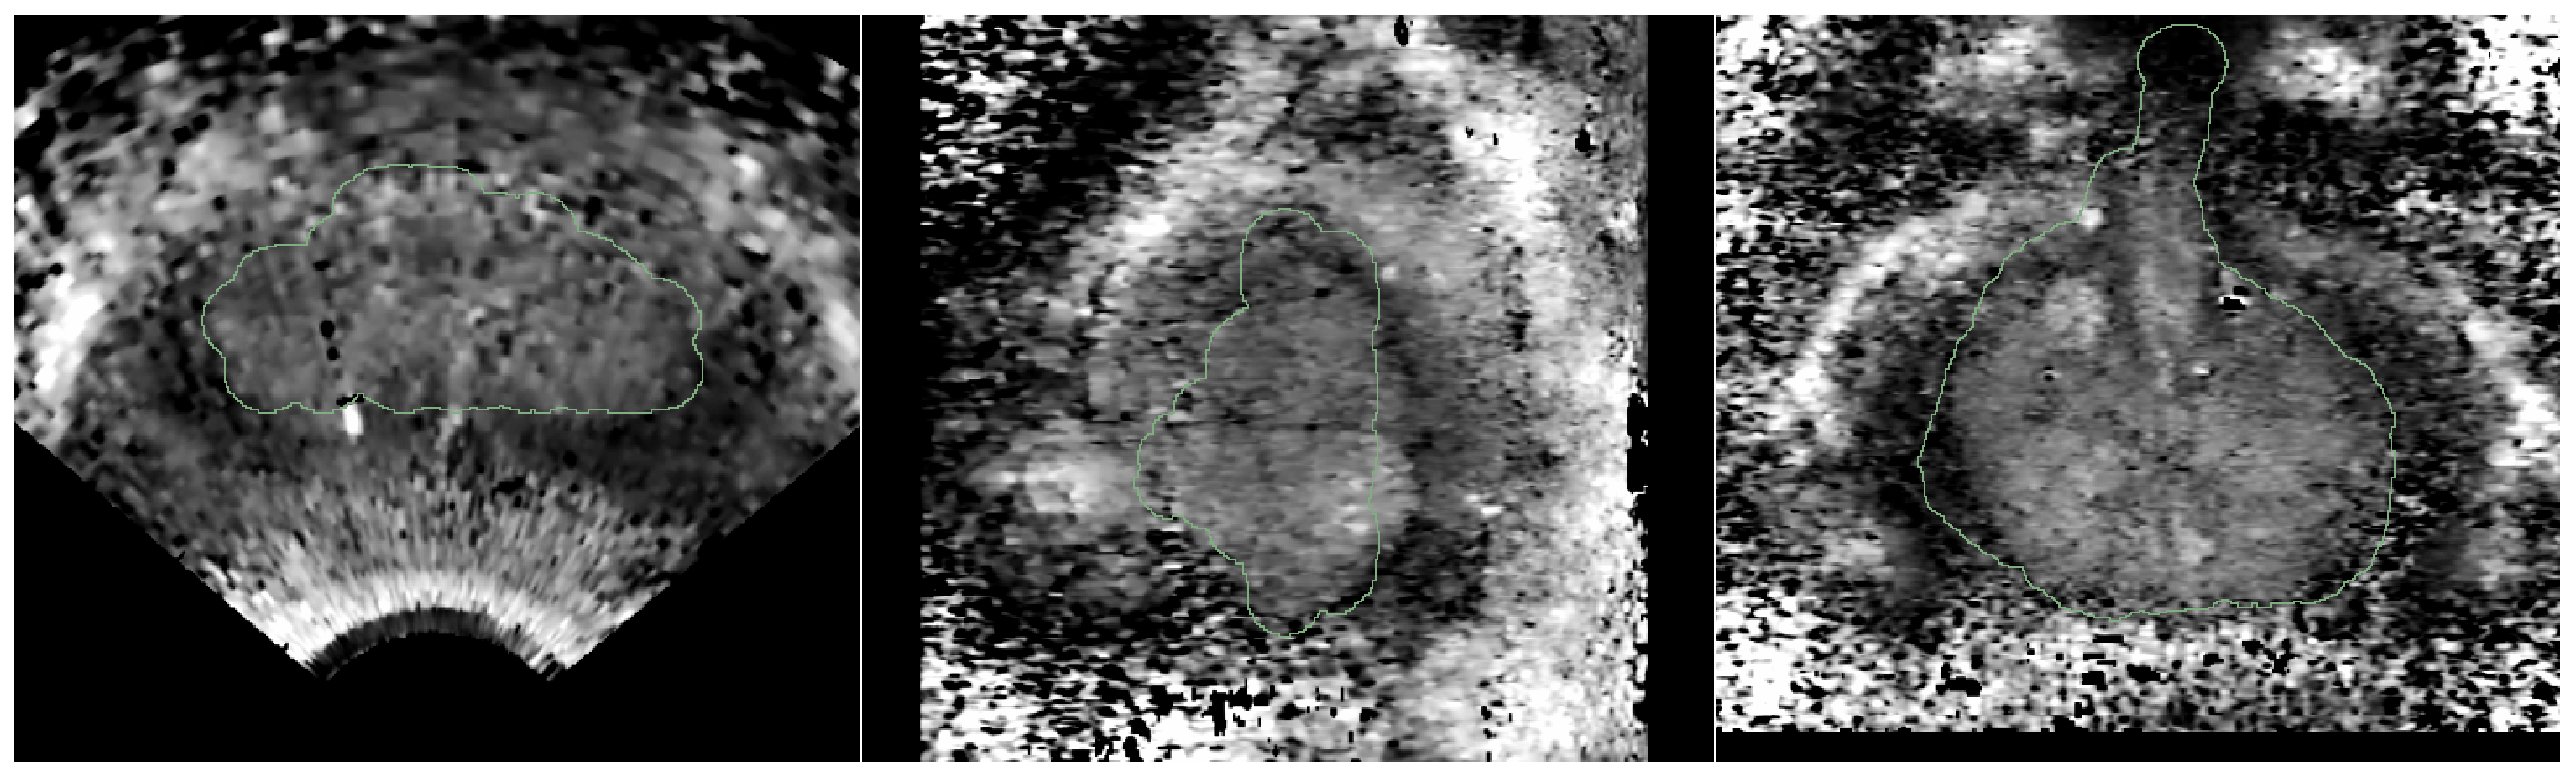
\includegraphics[width=1.0\textwidth]{figs/ARFI_CGsegs.eps} \\
\end{tabular}
\caption{Representative B-mode (top row) and ARFI images (bottom row), with
    superimposed segmentation outlines of the capsule and CG, respectively, for
    the same study subject shown in Figure~\ref{fig:mr_segs_vol}.  The B-mode
    images were segmented in the axial view, using the hypoechoic border of the
    capsule.  Notice that for large prostates, like the one shown in this
    figure, that the edges of the organ were not always captured in the imaging
    field-of-view.  The CG in the ARFI images was typically segmented using the
    coronal view, which, especially in the presence of extensive BPH, can have
    a very characteristic, heterogeneous appearance.  It should be noted that
    the coronal views in these ultrasound images are flipped 180\degree relative
    to the same images in Figure~\ref{fig:mr_segs_vol}.}
\label{fig:arfi_segs} 
\end{figure}


Segmented image stacks were imported into 3D Slicer (v4.3.0) and 3D
models were rendered using the following parameters (Table~\ref{tab:3dslicer}):

\begin{table}[h!]
\centering
\caption{3D model volume rendering parameters}
\begin{tabular}{ll}
{\bf Parameter} & {\bf Value} \\ \hline
Decimation & 0.1 \\
Smoothing Algorithm & Laplacian \\
Smoothing  & 70.0 \\
Joint Smoothing & Enabled \\
\end{tabular}
\label{tab:3dslicer}
\end{table}

The 3D slicer models were used to render volume estimates of the PZ and CG,
with the sum of PZ and CG representing the total prostate gland volume.  AFS
volume estimates in select MR cases were included in the total prostate gland
volume estimates.  Orthogonal tri-axial measurements in the lateral-to-lateral,
axex-to-base, and anterior-to-posterior dimensions were made in 3D slicer.
